% !TeX root = ../thuthesis-example.tex

\chapter{API优先开发}

API优先开发(API-First Development)是一种软件设计与开发方法论,其核心理念是在开始实际开发之前,优先设计、定义和确立应用程序接口(Application Programming Interface, API)。与传统的以用户界面或功能需求为起点的开发模式不同,API优先开发将API设计置于开发流程的最前端,使其成为系统架构和功能实现的基础。在API优先模式中,开发团队首先创建详细的API规范(通常采用OpenAPI/Swagger等标准),明确定义接口的资源、端点、请求方法、参数、响应格式以及身份验证机制等内容。

bolt.se的APIActions模块就是API优先开发理念的具体实现,它允许用户定义和管理外部API,并使LLM能够理解并使用这些API扩展功能。本章将详细介绍API优先开发的概念、意义、优势、对LLM驱动软件开发的重要性,以及bolt.se中APIActions的实现方案。

\section{API优先开发的概念与意义}

\subsection{API优先开发在软件工程中的优势}
API优先开发为现代软件工程带来了显著的优势:

\begin{enumerate}
  \item \textbf{并行开发效率}:明确的API规范使前端、后端和移动端团队能够在实际实现之前就达成共识,支持并行开发,减少集成阶段的冲突和返工。
  
  \item \textbf{一致性与标准化}:统一的API设计确保了系统中各服务接口的一致性,简化了学习曲线,降低了维护成本。
  
  \item \textbf{模块化与解耦}:以API为界面的系统设计促进了高内聚低耦合的架构,每个服务或模块仅需关注自身API的实现和消费,无需了解其他组件的内部逻辑。
  
  \item \textbf{可测试性增强}:明确的API规范使得在实现之前就可以进行接口测试设计,支持自动化测试和契约测试的实施。
  
  \item \textbf{文档驱动开发}:API规范自然成为系统的技术文档,减少了文档滞后或不准确的问题,提高了开发效率。
\end{enumerate}

在bolt.se这样的现代开发平台中,这些优势尤为明显,通过API优先方法减少了沟通成本、避免了误解并提早发现设计缺陷,显著提升了开发团队的整体效率和产品质量。

\subsection{API优先开发对LLM驱动软件开发的重要性}
在大型语言模型(LLM)驱动的软件开发范式中,API优先开发具有独特且关键的意义:

\begin{enumerate}
  \item \textbf{结构化信息交互}:LLM与外部系统和数据源交互需要明确的结构和规范。API定义为LLM提供了理解和正确调用外部服务的蓝图,避免了不精确指令可能导致的错误。
  
  \item \textbf{功能扩展与增强}:通过API集成,LLM可以突破其知识截止日期的限制,访问实时数据、专业工具和特定领域服务,大幅扩展其能力边界。
  
  \item \textbf{权限控制与安全管理}:API定义中的身份验证和授权机制,为LLM提供了受控的访问方式,确保其操作在安全和合规的边界内执行。
  
  \item \textbf{工具智能}(Tool Intelligence):预定义的API使LLM能够理解可用工具的能力和限制,做出更明智的工具选择和调用决策,实现"工具智能"。
  
  \item \textbf{实现可组合性}:API优先开发促进了LLM与各种服务和工具的组合使用,使复杂任务可以分解为多个API调用的组合,增强了问题解决能力。
\end{enumerate}

在bolt.se中,API优先理念已经深度融入系统设计。通过将OpenAPI规范直接集成到开发流程中,bolt.se实现了LLM与外部API的无缝协作,使开发者能够通过自然语言交互获得API增强的智能辅助。bolt.se的APIActions模块就是这一理念的具体实现,它允许用户定义和管理外部API,并使LLM能够理解并使用这些API扩展功能。这种结合不仅保留了LLM的灵活性和创造力,还增添了API的精确性和功能扩展性,为软件开发带来了革命性的效率提升。

\section{OpenAPI规范与API设计}
OpenAPI规范(原Swagger规范)是API优先开发方法论的核心技术支撑,它为API的描述和交互提供了一套标准化的、语言无关的格式\cite{openapi2023}。作为当前业界最广泛采用的API定义标准,OpenAPI使开发者能够以声明式的方式完整定义API的各个方面,从而实现从设计到实现、测试和文档的全生命周期管理。

OpenAPI规范采用JSON或YAML格式,以结构化的方式描述API的端点(endpoints)、操作(operations)、输入参数、输出响应、认证方法等关键要素。这种规范不仅能被人类理解,也可被机器处理,成为前端、后端和各种工具之间沟通的桥梁。

特别是在LLM驱动的开发环境中,OpenAPI规范以定义RESTful API调用说明,从而更高效地利用现有功能,避免重复开发,并降低大模型token使用。这是因为结构化的API定义使大模型能够:
\begin{enumerate}
  \item 准确理解API的功能和用法,无需详细的自然语言解释
  \item 通过直接调用现有API获取数据,而非生成可能不准确的信息
  \item 避免在上下文中包含冗长的API使用说明,节省宝贵的token空间
  \item 将复杂任务分解为定义明确的API调用序列,提高解决问题的效率
\end{enumerate}

\subsection{OpenAPI规范简介}
OpenAPI规范是一个结构化的API描述格式,具有以下主要组成部分\cite{openapi2023spec}:

\begin{enumerate}
  \item \textbf{基本信息}:包括API的标题、描述、版本、联系人信息和许可证等元数据。
  
  \item \textbf{服务器信息}:定义API的基础URL和可能的不同环境(如开发、测试、生产)的服务器地址。
  
  \item \textbf{路径}:描述API的各个端点及其可用的HTTP方法(GET、POST、PUT、DELETE等),是规范的核心部分。
  
  \item \textbf{组件}:包含可重用的部分:
    \begin{itemize}
      \item \textit{schemas}:定义API使用的数据模型和对象结构。
      \item \textit{parameters}:定义可重用的参数定义。
      \item \textit{responses}:定义各种响应格式和状态码。
      \item \textit{securitySchemes}:描述API支持的安全认证机制。
    \end{itemize}
  
  \item \textbf{操作}:每个API端点可用的操作,包括:
    \begin{itemize}
      \item 操作ID与摘要,用于工具和代码生成。
      \item 详细描述与标签,用于文档组织。
      \item 参数定义(路径、查询、头部、cookie等)。
      \item 请求体结构与格式。
      \item 可能的响应状态与内容。
      \item 所需的安全机制。
    \end{itemize}
\end{enumerate}

以下是bolt.se中支持的OpenAPI定义示例,展示了一个简单的天气API:

\begin{verbatim}
openapi: 3.0.0
info:
  title: Weather API
  version: 1.0.0
servers:
  - url: https://api.weather.gov
    description: Weather API Server
paths:
  /weather/current:
    get:
      summary: Get current weather
      parameters:
        - name: city
          in: query
          required: true
          schema:
            type: string
      responses:
        '200':
          description: Current weather data
          content:
            application/json:
              schema:
                type: object
                properties:
                  temperature:
                    type: number
                  conditions:
                    type: string
\end{verbatim}

bolt.se的APIActions模块能够解析这种OpenAPI定义,自动提取API端点和操作,使LLM能够理解并正确调用这些API。

\subsection{使用OpenAPI规范进行API设计的优势}
在bolt.se这样的现代开发环境中,采用OpenAPI规范进行API设计带来了多方面的显著优势:

\begin{enumerate}
  \item \textbf{设计驱动开发}:OpenAPI规范促使开发者在编写代码前先思考接口设计,从需求和用户体验出发设计API,避免了实现细节对接口设计的不当影响。
  
  \item \textbf{自动化代码生成}:基于OpenAPI规范,bolt.se可以帮助开发者生成调用API的代码片段,减少重复编码工作,提高开发效率。
  
  \item \textbf{交互式使用}:bolt.se将OpenAPI规范转化为可交互的形式,使用户能够通过自然语言请求直接调用这些API,无需编写复杂的代码。
    
  \item \textbf{机器可读性}:规范的结构化特性使LLM能够理解和分析API,为智能开发辅助、代码补全和自动化请求提供了基础。
\end{enumerate}

在bolt.se中,OpenAPI规范的机器可读特性具有重要价值。LLM可以基于规范生成准确的API调用代码,理解API的功能边界,甚至可以提供API使用建议。同时,规范中明确的数据模型和参数约束有助于LLM生成更准确的代码和请求,减少错误和误解。

bolt.se的APIActions模块不仅用于定义系统内部的服务接口,也被用作用户自定义外部API的标准格式。通过将OpenAPI文档直接解析为系统理解的API操作集,bolt.se实现了让大语言模型直接利用这些API进行交互和代码生成,展示了API优先理念与AI驱动开发的深度融合。

\section{bolt.se中的APIActions实现}
bolt.se作为一个AI驱动的软件开发平台,将API优先开发理念深度融入其架构设计。系统通过结构化的APIActions模块,使用户能够轻松定义、管理和应用外部API,同时让大语言模型能够理解并调用这些API,实现功能扩展和技术集成。本节将详细介绍bolt.se中APIActions的实现方案,从整体架构设计到具体功能实现。

\begin{figure}[htbp]
  \centering
  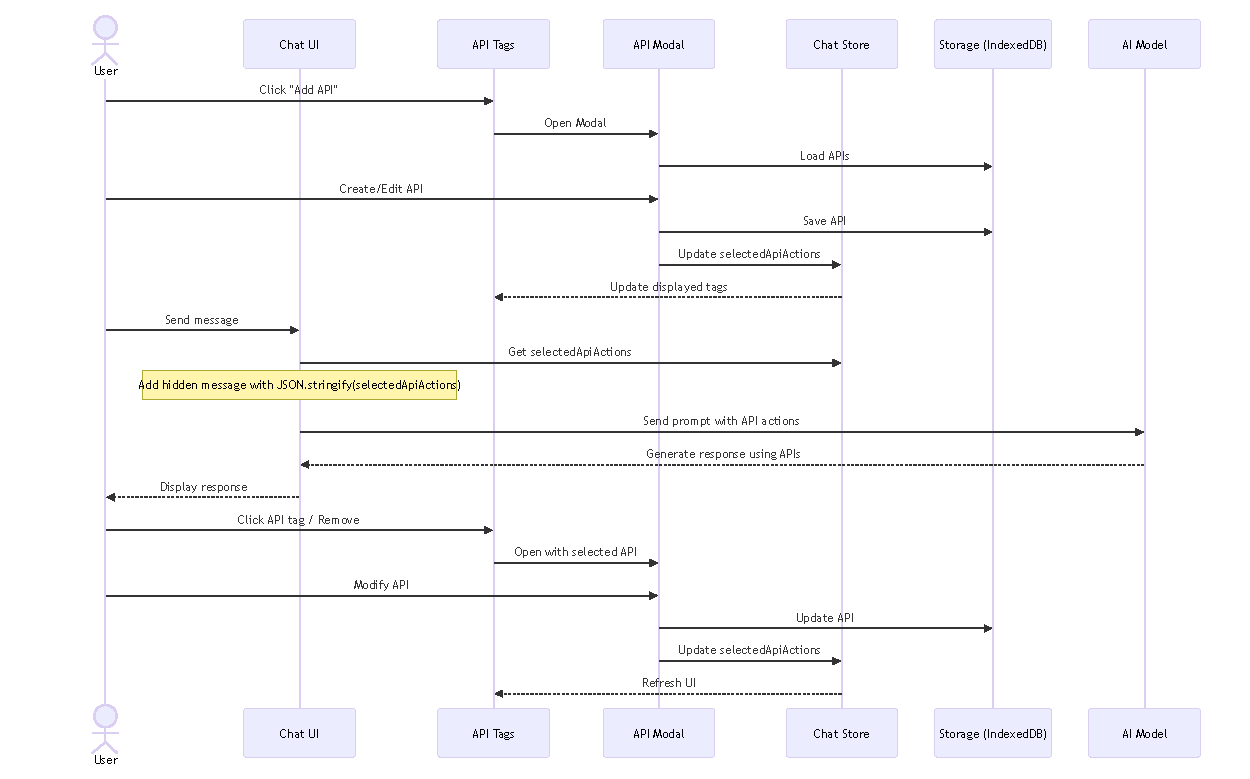
\includegraphics[width=\textwidth]{figures/api_workflow.pdf}
  \caption{API使用工作流程图:展示了用户创建、编辑和使用API的完整流程,以及API信息如何在系统各组件间传递}
  \label{fig:api_workflow}
\end{figure}

\subsection{APIActions与Token效率优化}
在LLM应用开发过程中,token使用效率是一个关键考量因素,直接影响到系统的响应速度、成本和可扩展性。bolt.se的APIActions模块通过OpenAPI规范的结构化定义,显著提升了token使用效率:

\begin{enumerate}
  \item \textbf{精简上下文传递}:APIActions将API完整功能通过结构化格式传递给LLM,相比使用自然语言描述全部API功能,可以节省高达70\%的token消耗。例如,一个包含50个端点的API,使用OpenAPI描述可能仅需约2000个token,而详细的自然语言描述可能需要6000-8000个token。
  
  \item \textbf{减少幻觉生成}:通过APIActions,LLM可以直接调用外部服务获取准确信息,避免因知识截止日期限制而产生的幻觉内容,同时减少了用于生成猜测内容的token消耗。
  
  \item \textbf{简化指令结构}:结构化的API定义使LLM能够轻松理解可用操作,无需开发者提供冗长的指示说明,从而在对话上下文中节省token空间。
  
  \item \textbf{最小化迭代次数}:清晰的API定义减少了LLM理解和使用API所需的交互次数,每减少一轮交互就可能节省数百甚至数千个token。
\end{enumerate}

bolt.se在复杂的开发任务中,使用APIActions可以比传统方法减少token消耗,同时提高结果的准确性和一致性。这种效率提升对于大规模应用部署和持续使用尤为重要,直接转化为运营成本的显著降低。

\subsection{整体架构设计与模块划分}
bolt.se的APIActions系统采用了模块化设计,主要由以下几个核心组件构成:

\begin{enumerate}
  \item \textbf{用户界面组件}:
    \begin{itemize}
      \item \texttt{ApiActionsContextTags}:显示在聊天界面中选中的API标签
      \item \texttt{ApiActionsModal}:管理API的主要模态窗口
      \item \texttt{EditApiActionsModal}:创建和编辑API的编辑器界面
    \end{itemize}
  
  \item \textbf{数据管理组件}:
    \begin{itemize}
      \item \texttt{chatStore}:管理当前聊天中选中的API(selectedApiActions)
      \item \texttt{useApiActions}:提供API的增删改查功能的React Hook
      \item \texttt{IndexedDB存储}:持久化存储API定义
    \end{itemize}
  
  \item \textbf{AI交互层}:负责将选定的API信息传递给大语言模型,并处理模型的响应结果。
\end{enumerate}

如图\ref{fig:api_workflow}所示,整个API使用流程分为三个主要阶段:API创建与管理、在对话中使用API以及API的编辑与移除。这种设计确保了API的全生命周期管理,从定义到使用再到维护的完整闭环。

在数据模型设计方面,bolt.se定义了结构化的API数据模型,如图\ref{fig:api_actions_class}所示。核心数据结构是ApiActions类,它包含API的所有必要信息:

\begin{figure}[htbp]
  \centering
  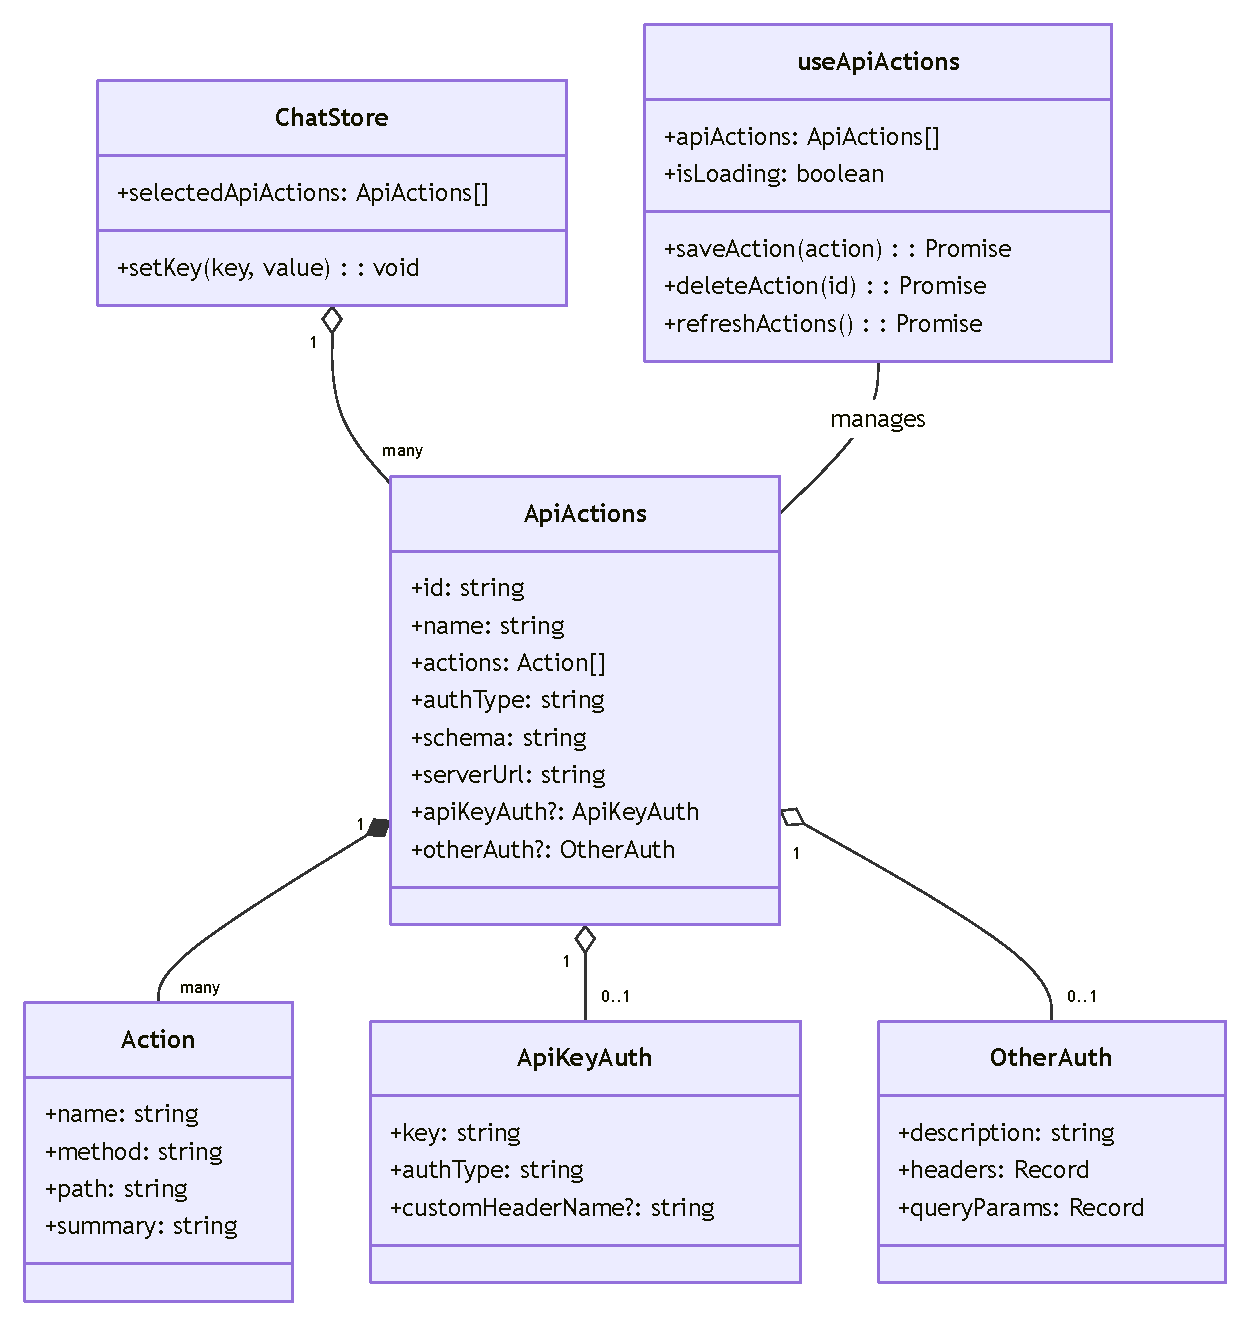
\includegraphics[width=\textwidth]{figures/api_actions_class.pdf}
  \caption{API数据模型类图:描述了系统中API定义的核心数据结构及其关系,包括API操作、认证方式和存储管理}
  \label{fig:api_actions_class}
\end{figure}

ApiActions数据模型的主要组成包括:

\begin{enumerate}
  \item \textbf{基本信息}:包括唯一标识符(id)、名称(name)和基础URL(serverUrl)。
  
  \item \textbf{API操作集}:由多个Action对象组成,每个Action定义了一个API端点的HTTP方法、路径和功能摘要。
  
  \item \textbf{认证信息}:支持三种认证方式:
    \begin{itemize}
      \item \texttt{none}:无需认证的API
      \item \texttt{apiKey}:通过API密钥认证,支持Basic、Bearer或自定义头部方式
      \item \texttt{other}:其他自定义认证,可配置自定义头部和查询参数
    \end{itemize}
  
  \item \textbf{OpenAPI规范}:通过schema字段存储完整的OpenAPI规范定义,为系统提供API的详细信息。
\end{enumerate}

bolt.se的APIActions模块具有以下关键功能:

\begin{enumerate}
  \item \textbf{OpenAPI解析与提取}:系统能够解析OpenAPI规范,自动识别并提取API端点、方法和参数,减少用户配置负担。
  
  \item \textbf{多种认证支持}:灵活支持不同API认证方式,包括无认证、API密钥(Bearer、Basic、自定义头部)和其他自定义认证方式。
  
  \item \textbf{API标签系统}:通过标签化展示选中的API,提供直观的视觉反馈,方便管理多个API。
  
  \item \textbf{实时编辑与更新}:支持API定义的实时编辑和更新,变更立即反映在对话中。
  
  \item \textbf{LLM集成机制}:将选中的API信息以结构化形式注入LLM上下文,使模型能够理解并正确调用这些API。
\end{enumerate}

\section{实例应用场景}

本节以一个聊天机器人应用为例,展示在 \emph{bolt.se} 中如何使用
APIActions 模块集成多个外部 API,并借助 LLM 实现任务规划、
代码生成与界面交互的全过程。该机器人能够回答天气相关问题并展示狗狗图片,
集成了 OpenAI API、NWS Weather API 与 The Dog API。

\subsection{添加与配置 APIActions}

用户首先通过图形界面进入 APIActions 模块(如图 \ref{fig:demo_edit}),
粘贴 OpenAPI 定义并选择认证方式。以 NWS Weather API 为例,
其提供了两个操作端点,分别用于获取经纬度对应的网格点与天气预报:

\begin{figure}[htbp]
  \centering
  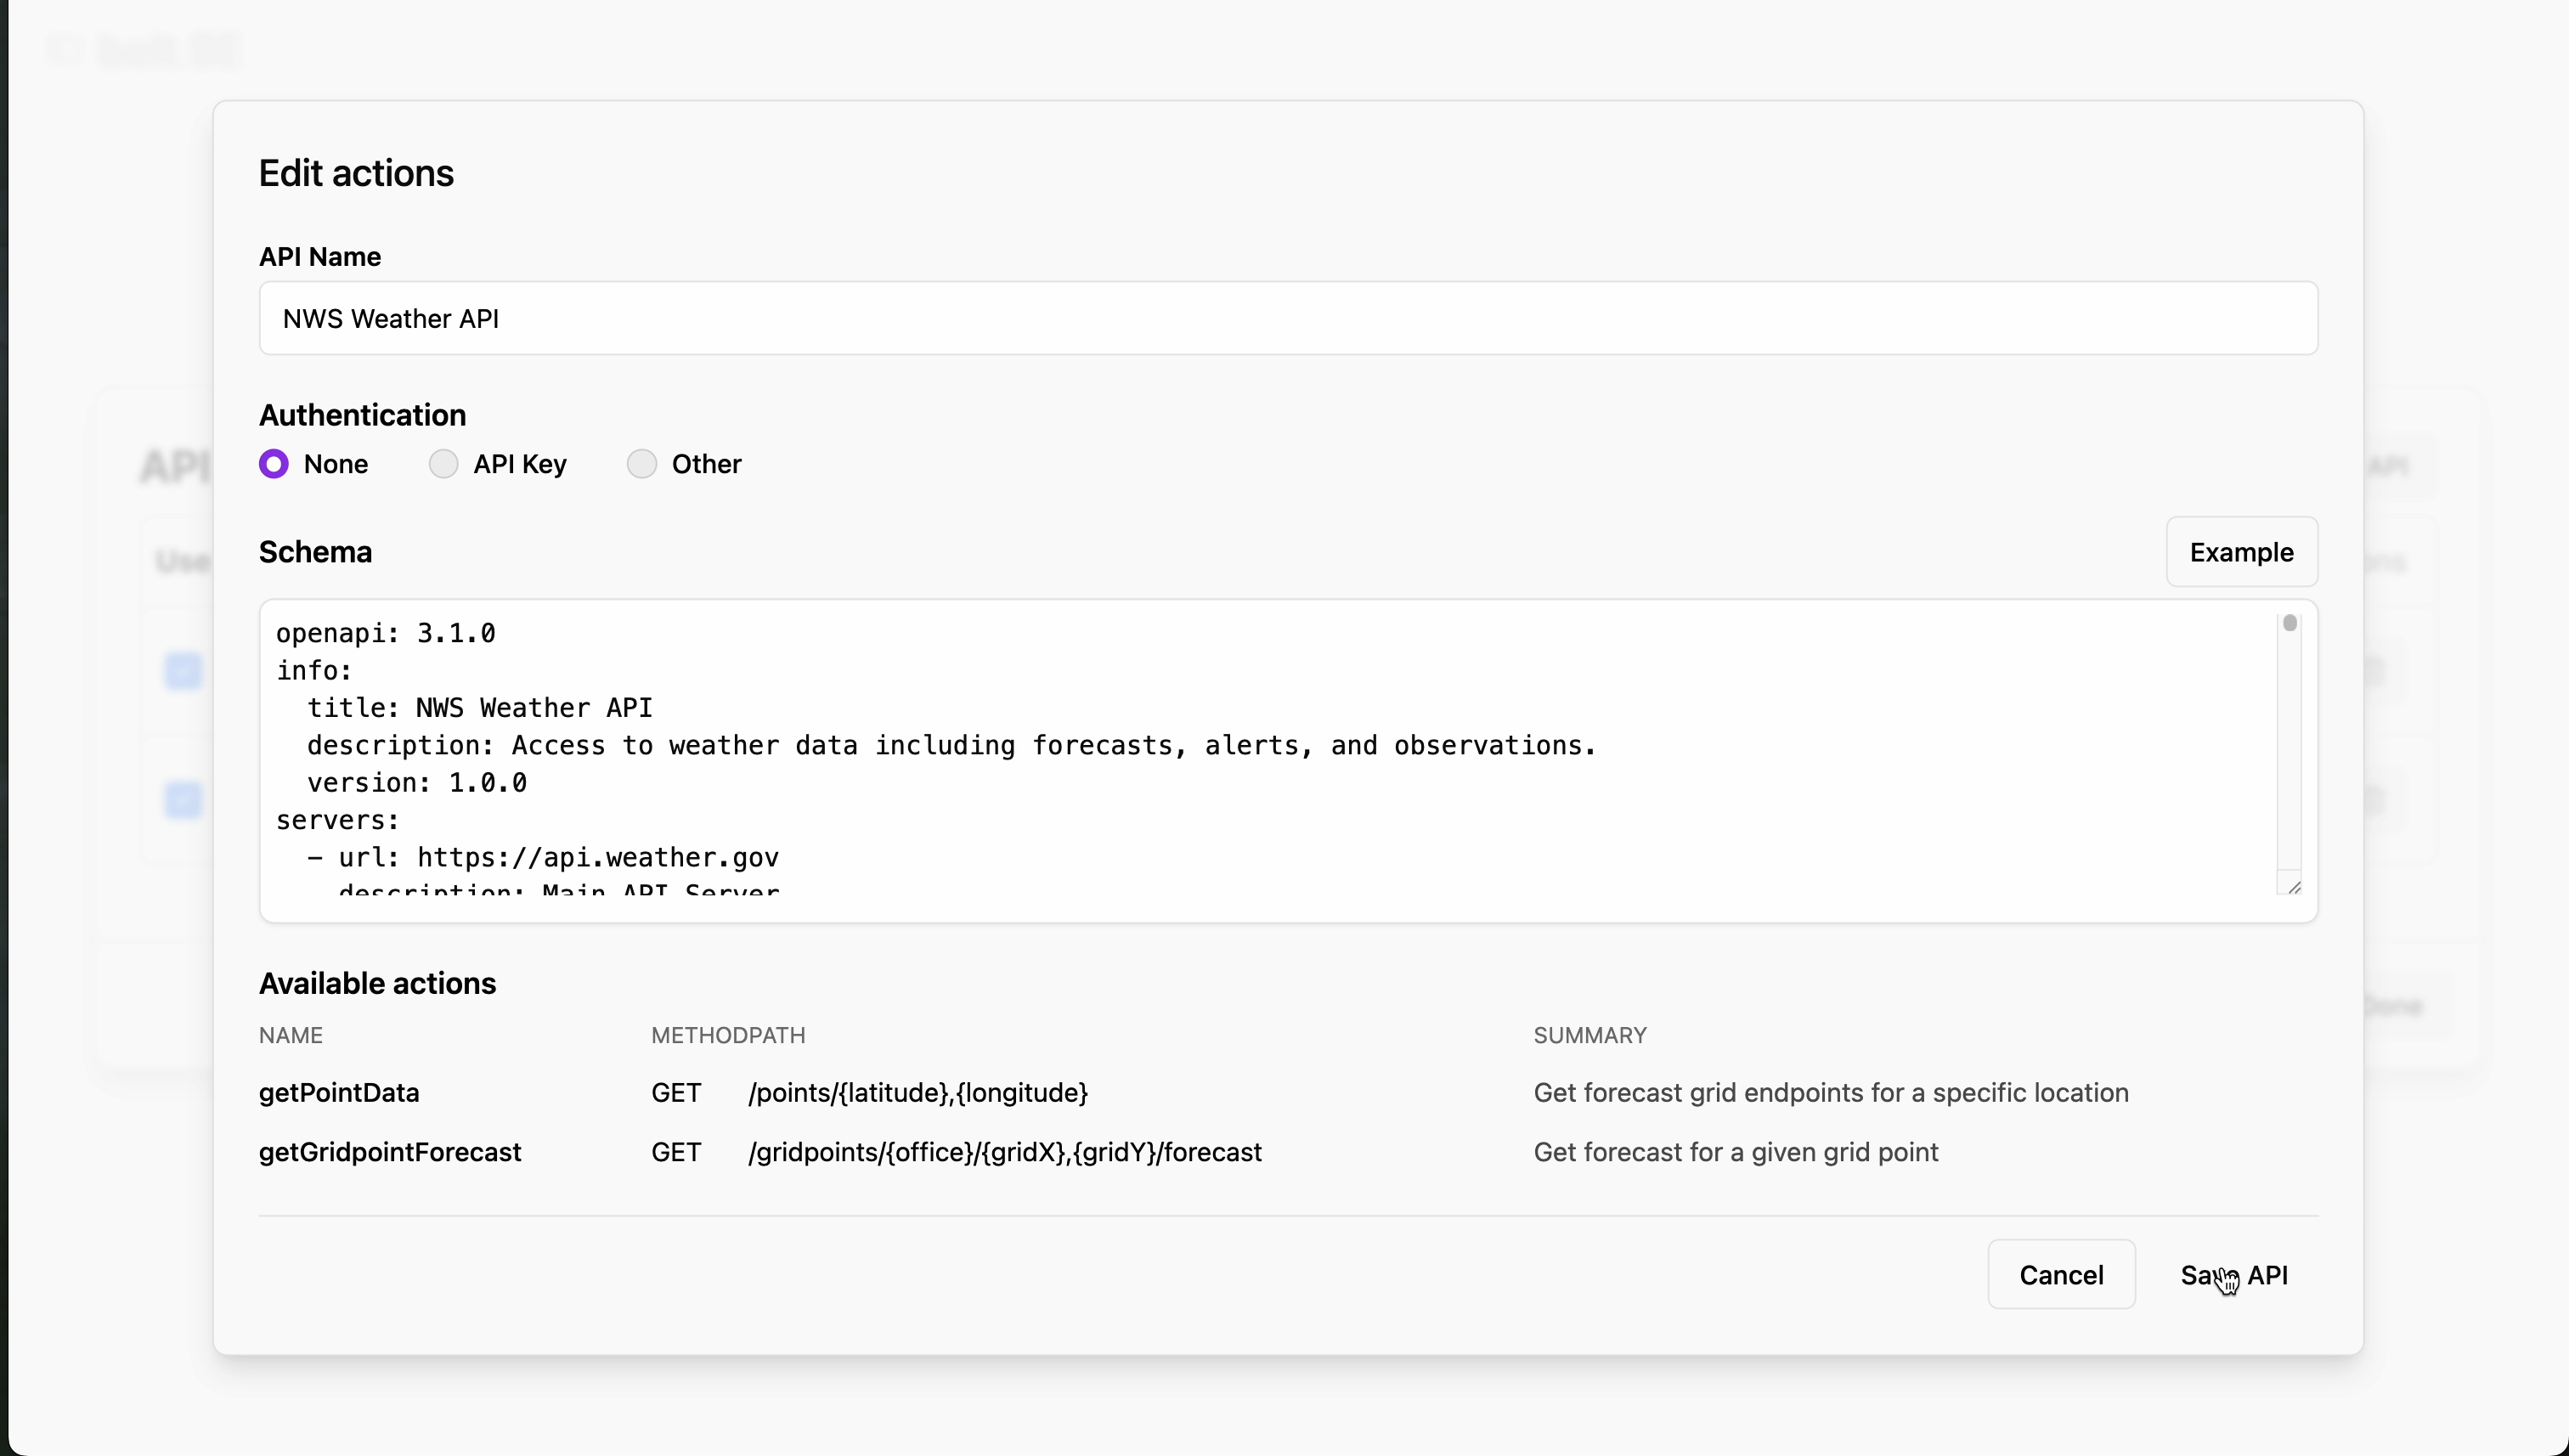
\includegraphics[width=\textwidth]{figures/screenshots/api-actions/demo_edit_modal.png}
  \caption{添加 NWS Weather API:通过粘贴 OpenAPI 规范定义并配置端点与认证方式。}
  \label{fig:demo_edit}
\end{figure}

配置完成后,用户可以在 APIActions 列表中启用或禁用对应 API,
系统也支持随时编辑、删除、重载 schema(如图 \ref{fig:demo_table})。

\begin{figure}[htbp]
  \centering
  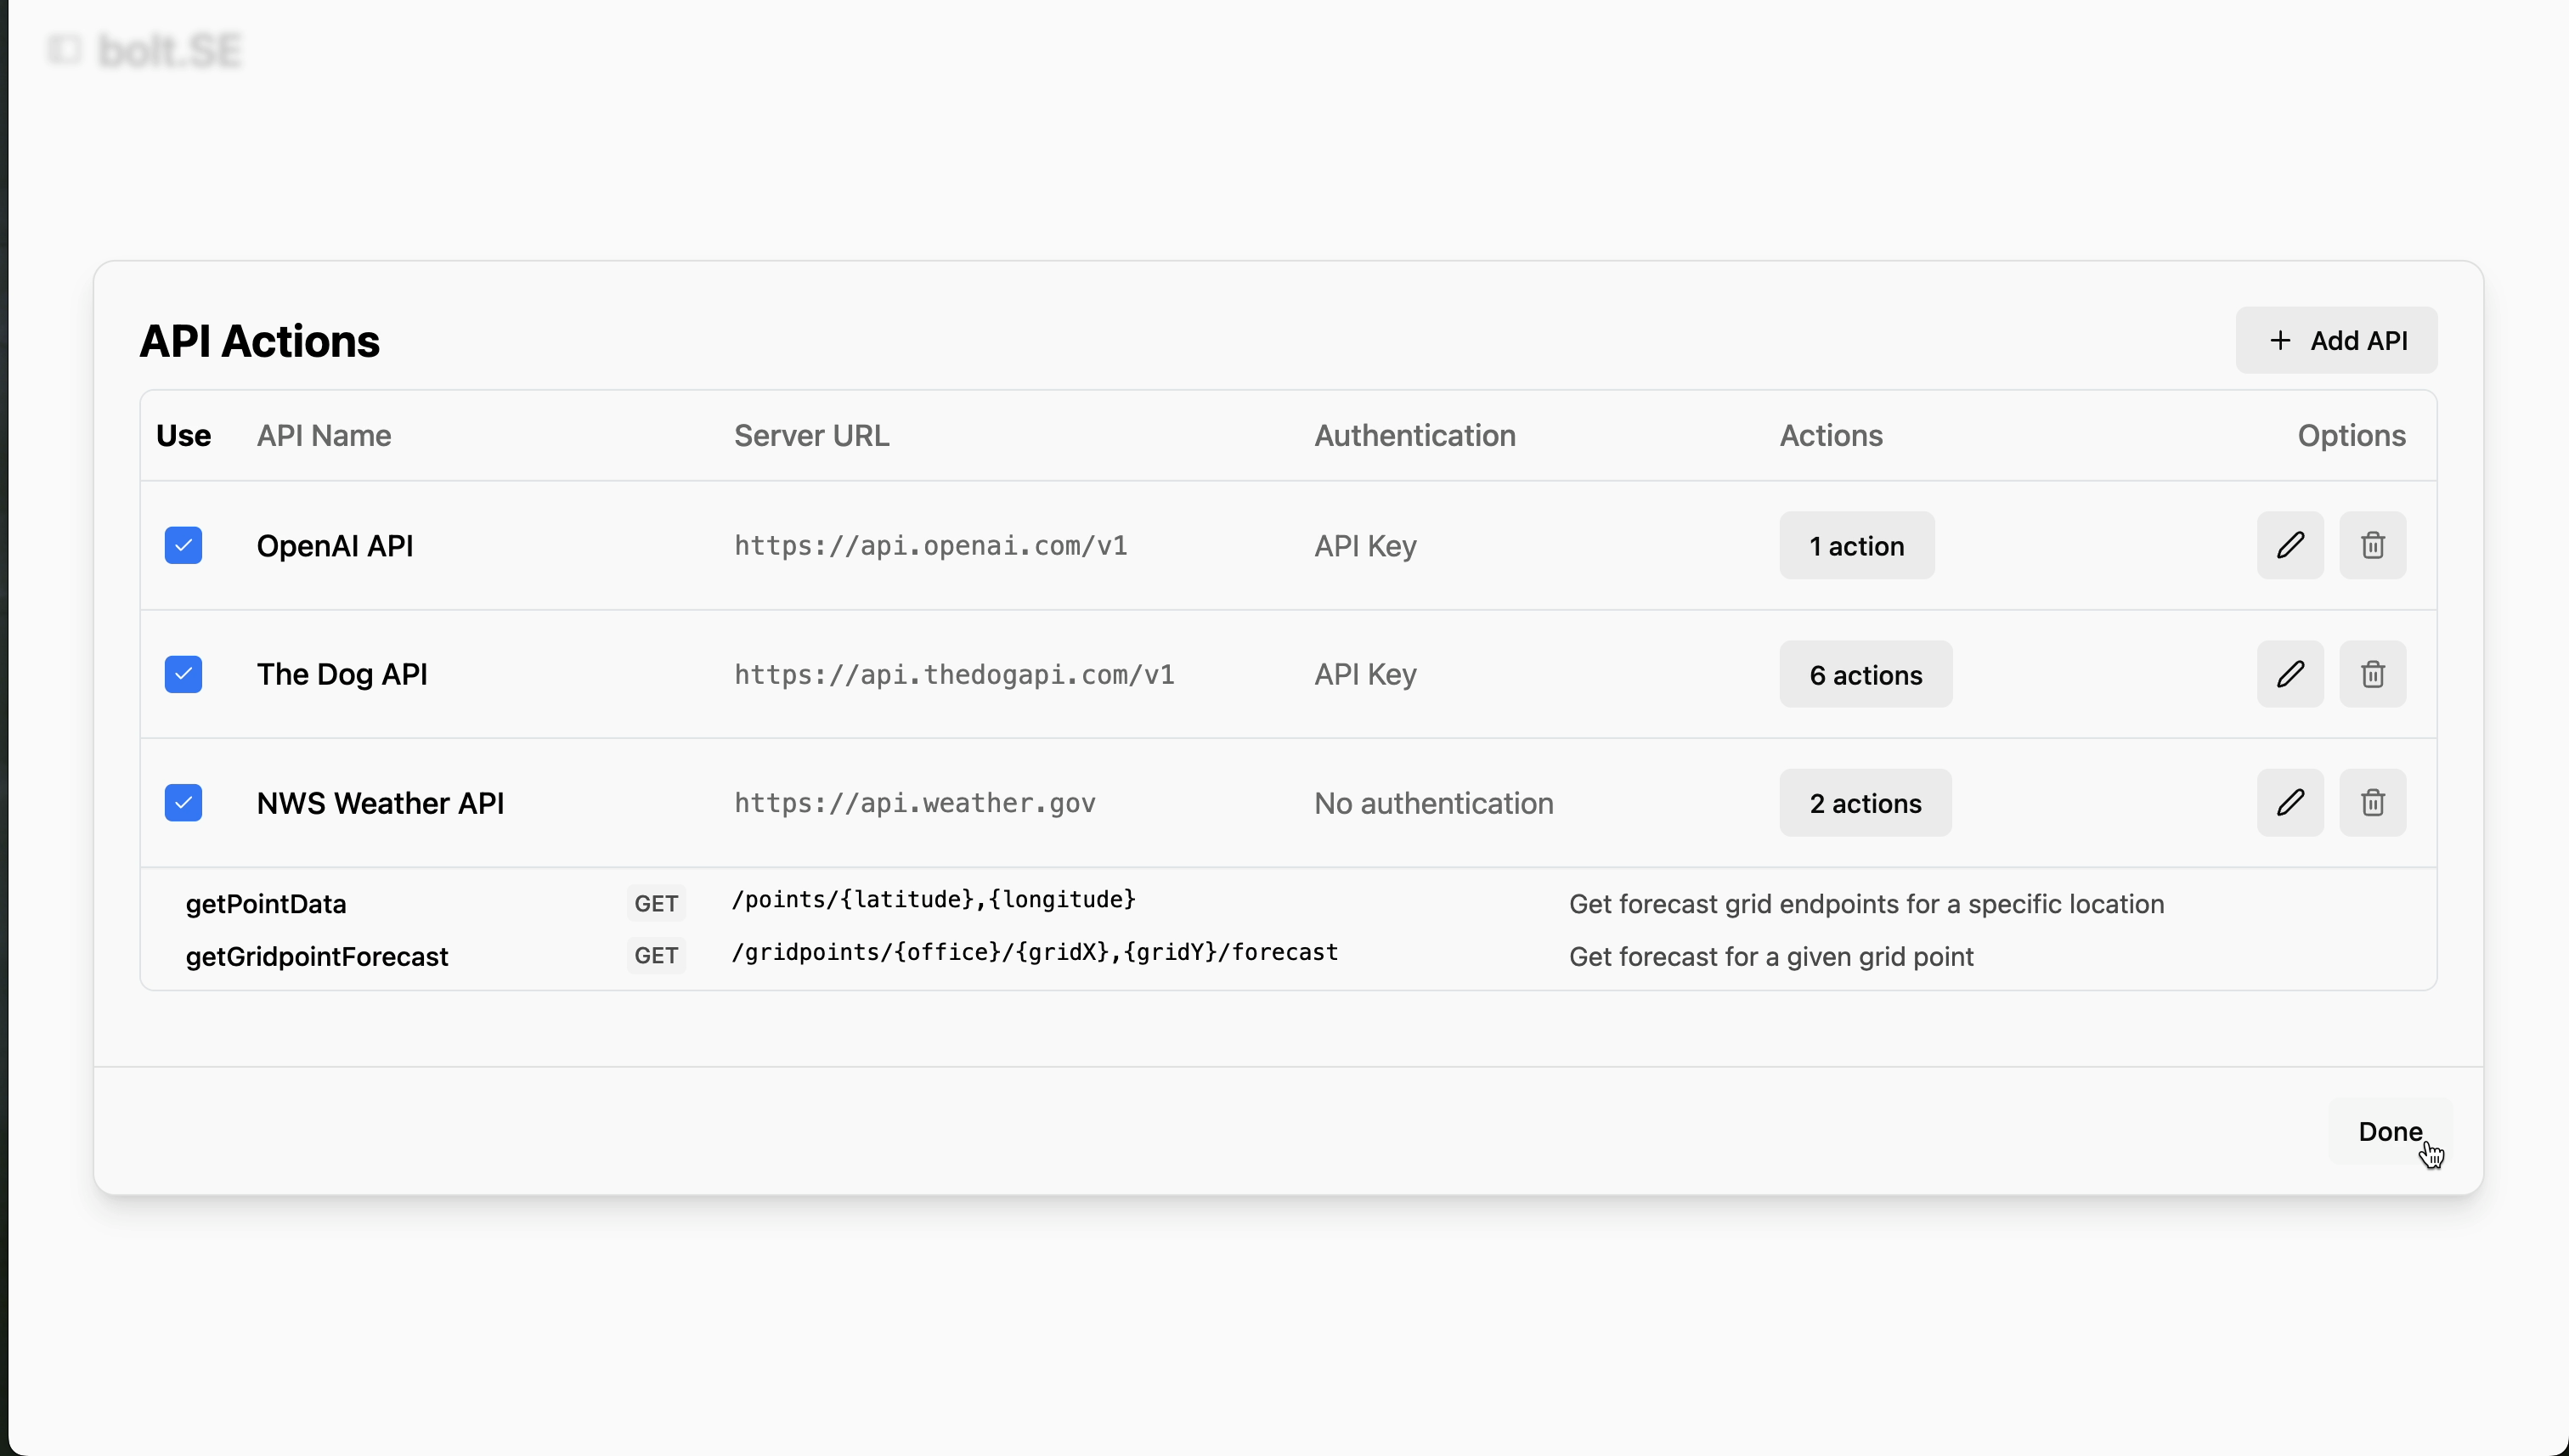
\includegraphics[width=\textwidth]{figures/screenshots/api-actions/demo_actions_table.png}
  \caption{APIActions 总览界面:展示所有注册的 API、认证方式与可用操作数。}
  \label{fig:demo_table}
\end{figure}

\subsection{自然语言触发任务规划与代码生成}

完成 API 配置后,用户可在主对话框中勾选所需 API(如图 \ref{fig:demo_prompt}),
并以自然语言输入构想,例如:

\begin{quote}
\texttt{make a chatbot that can answer weather related questions and show dog images}
\end{quote}

\begin{figure}[htbp]
  \centering
  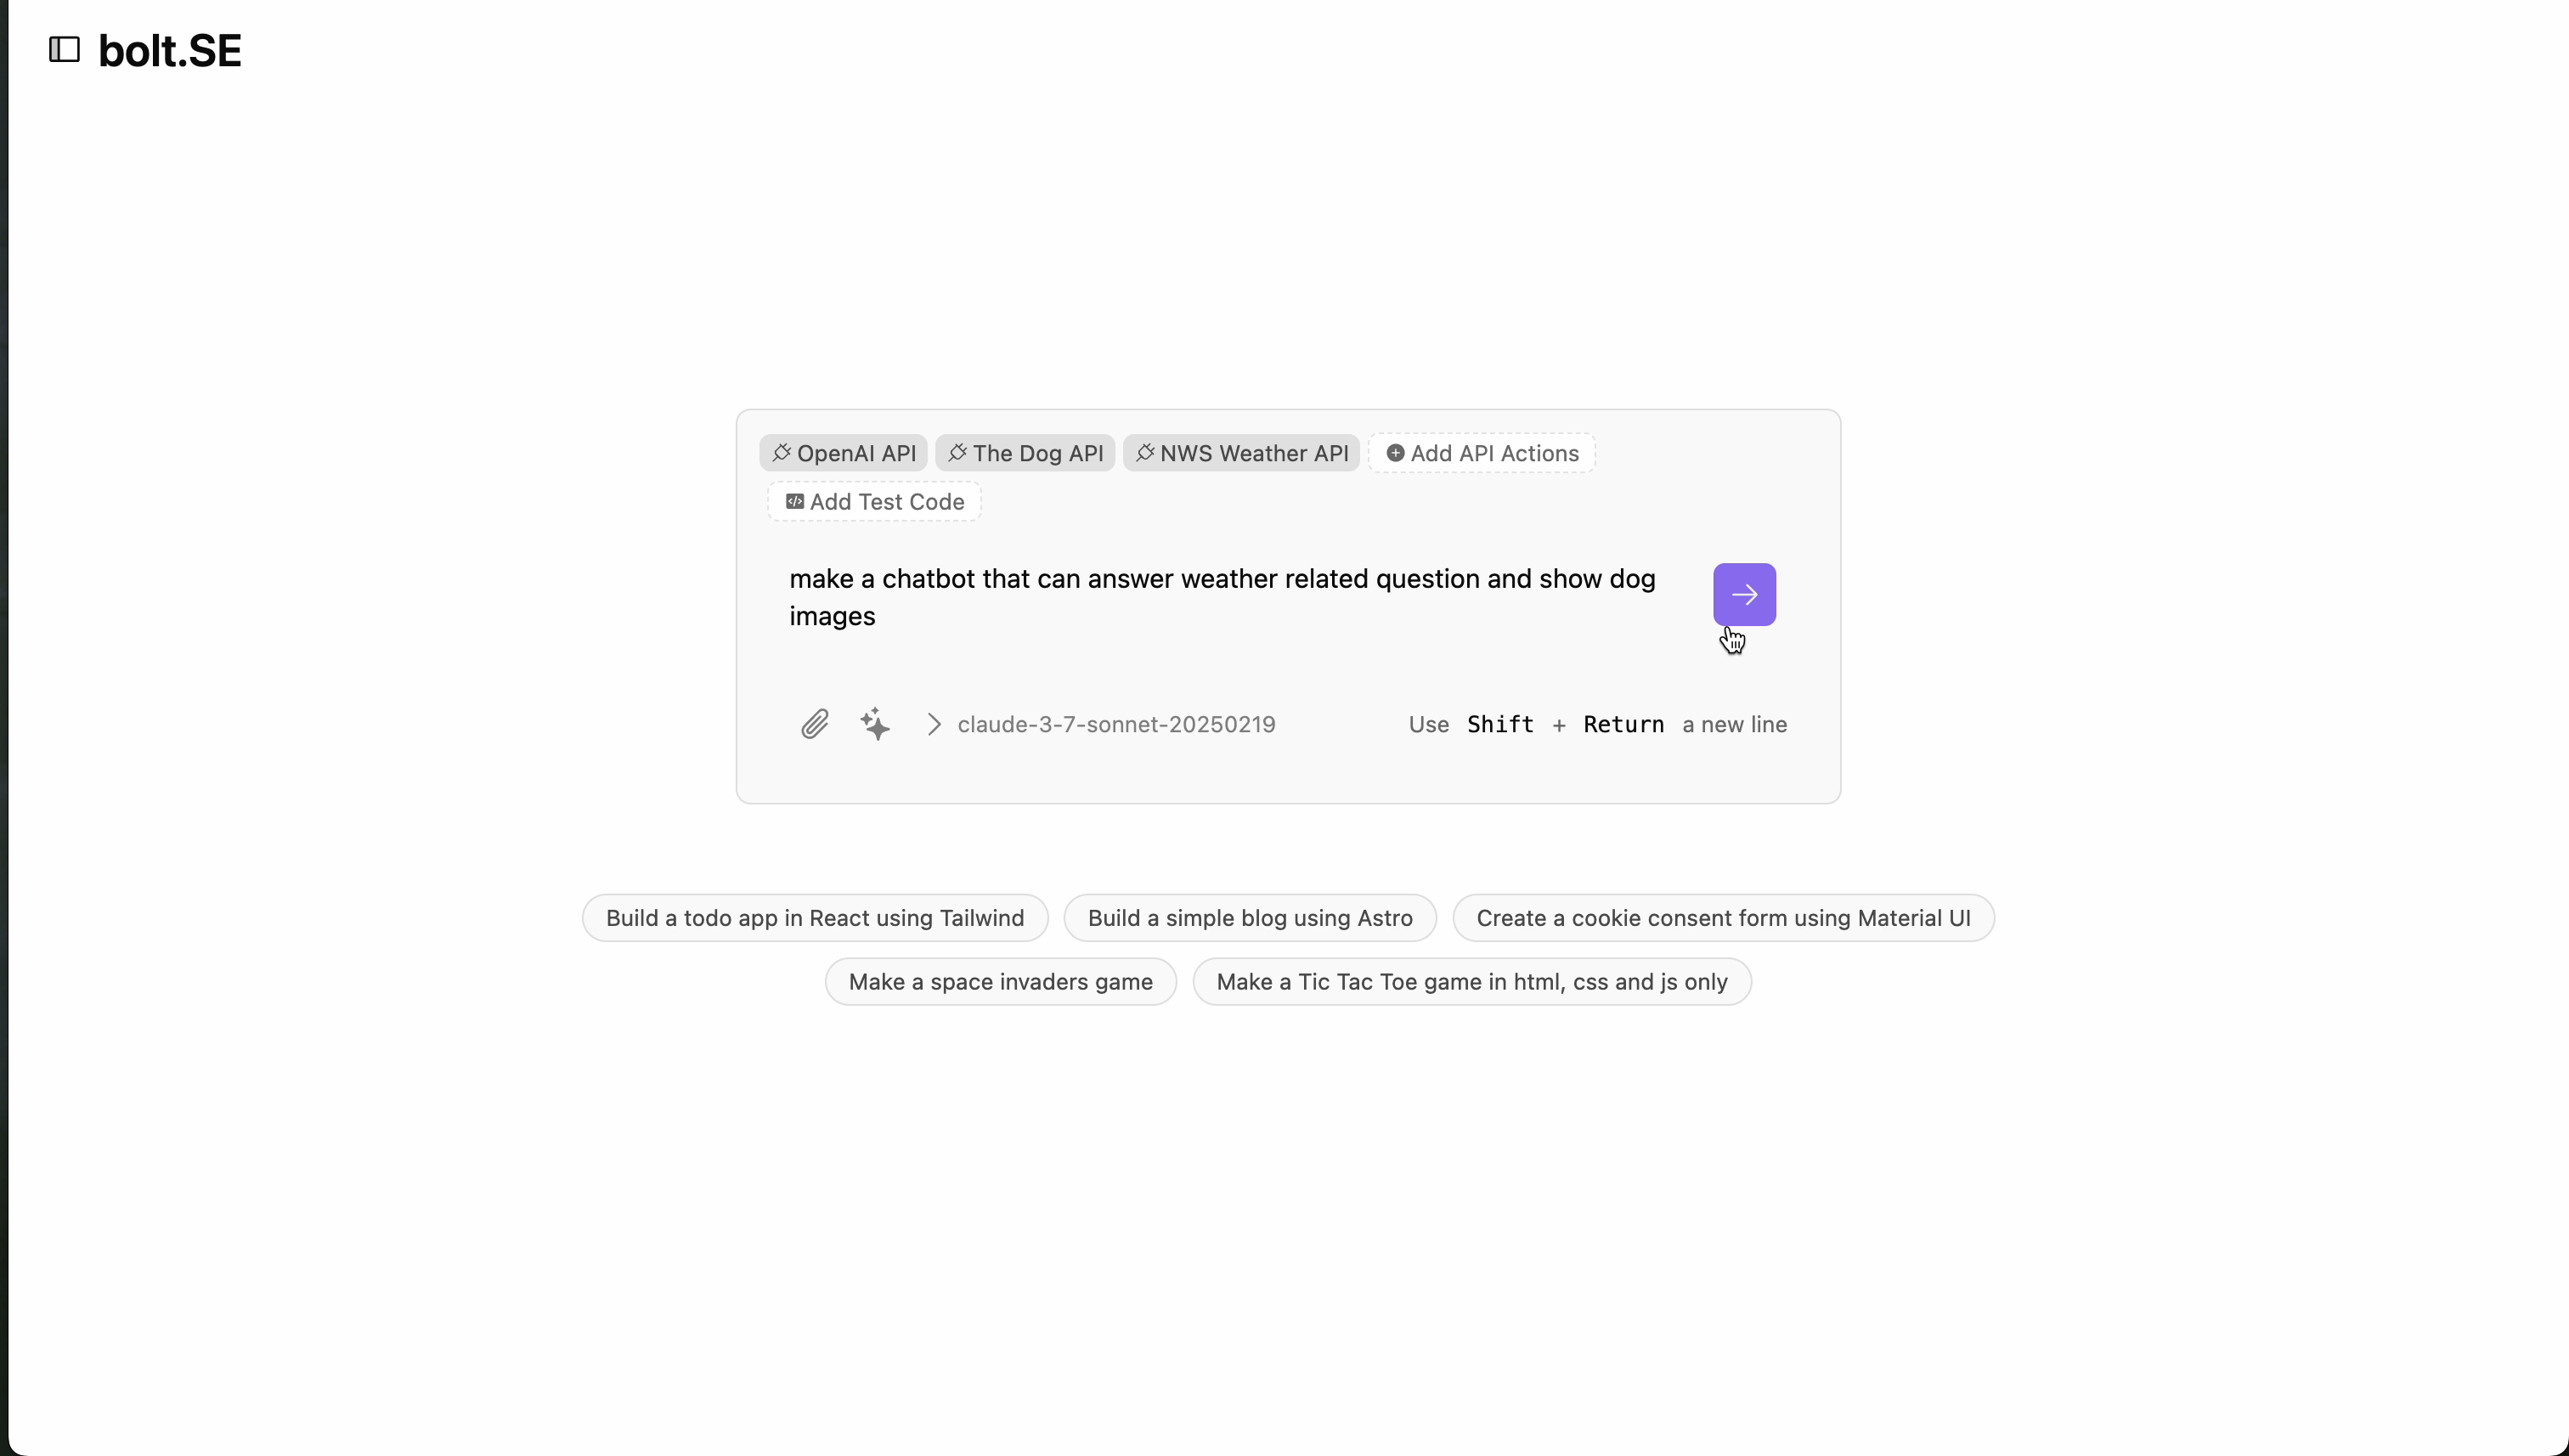
\includegraphics[width=\textwidth]{figures/screenshots/api-actions/demo_prompt_tags.png}
  \caption{对话框中勾选相关 API,配合自然语言指令触发任务生成。}
  \label{fig:demo_prompt}
\end{figure}

系统会基于勾选的 API 及用户意图,自动规划任务、生成文件,并提示相关操作步骤。

\subsection{代码结构与依赖初始化}

如图 \ref{fig:demo_plan} 所示,bolt.se 自动列出开发计划并实时创建必要的文件结构。
同时生成项目依赖清单与安装命令。

\begin{figure}[htbp]
  \centering
  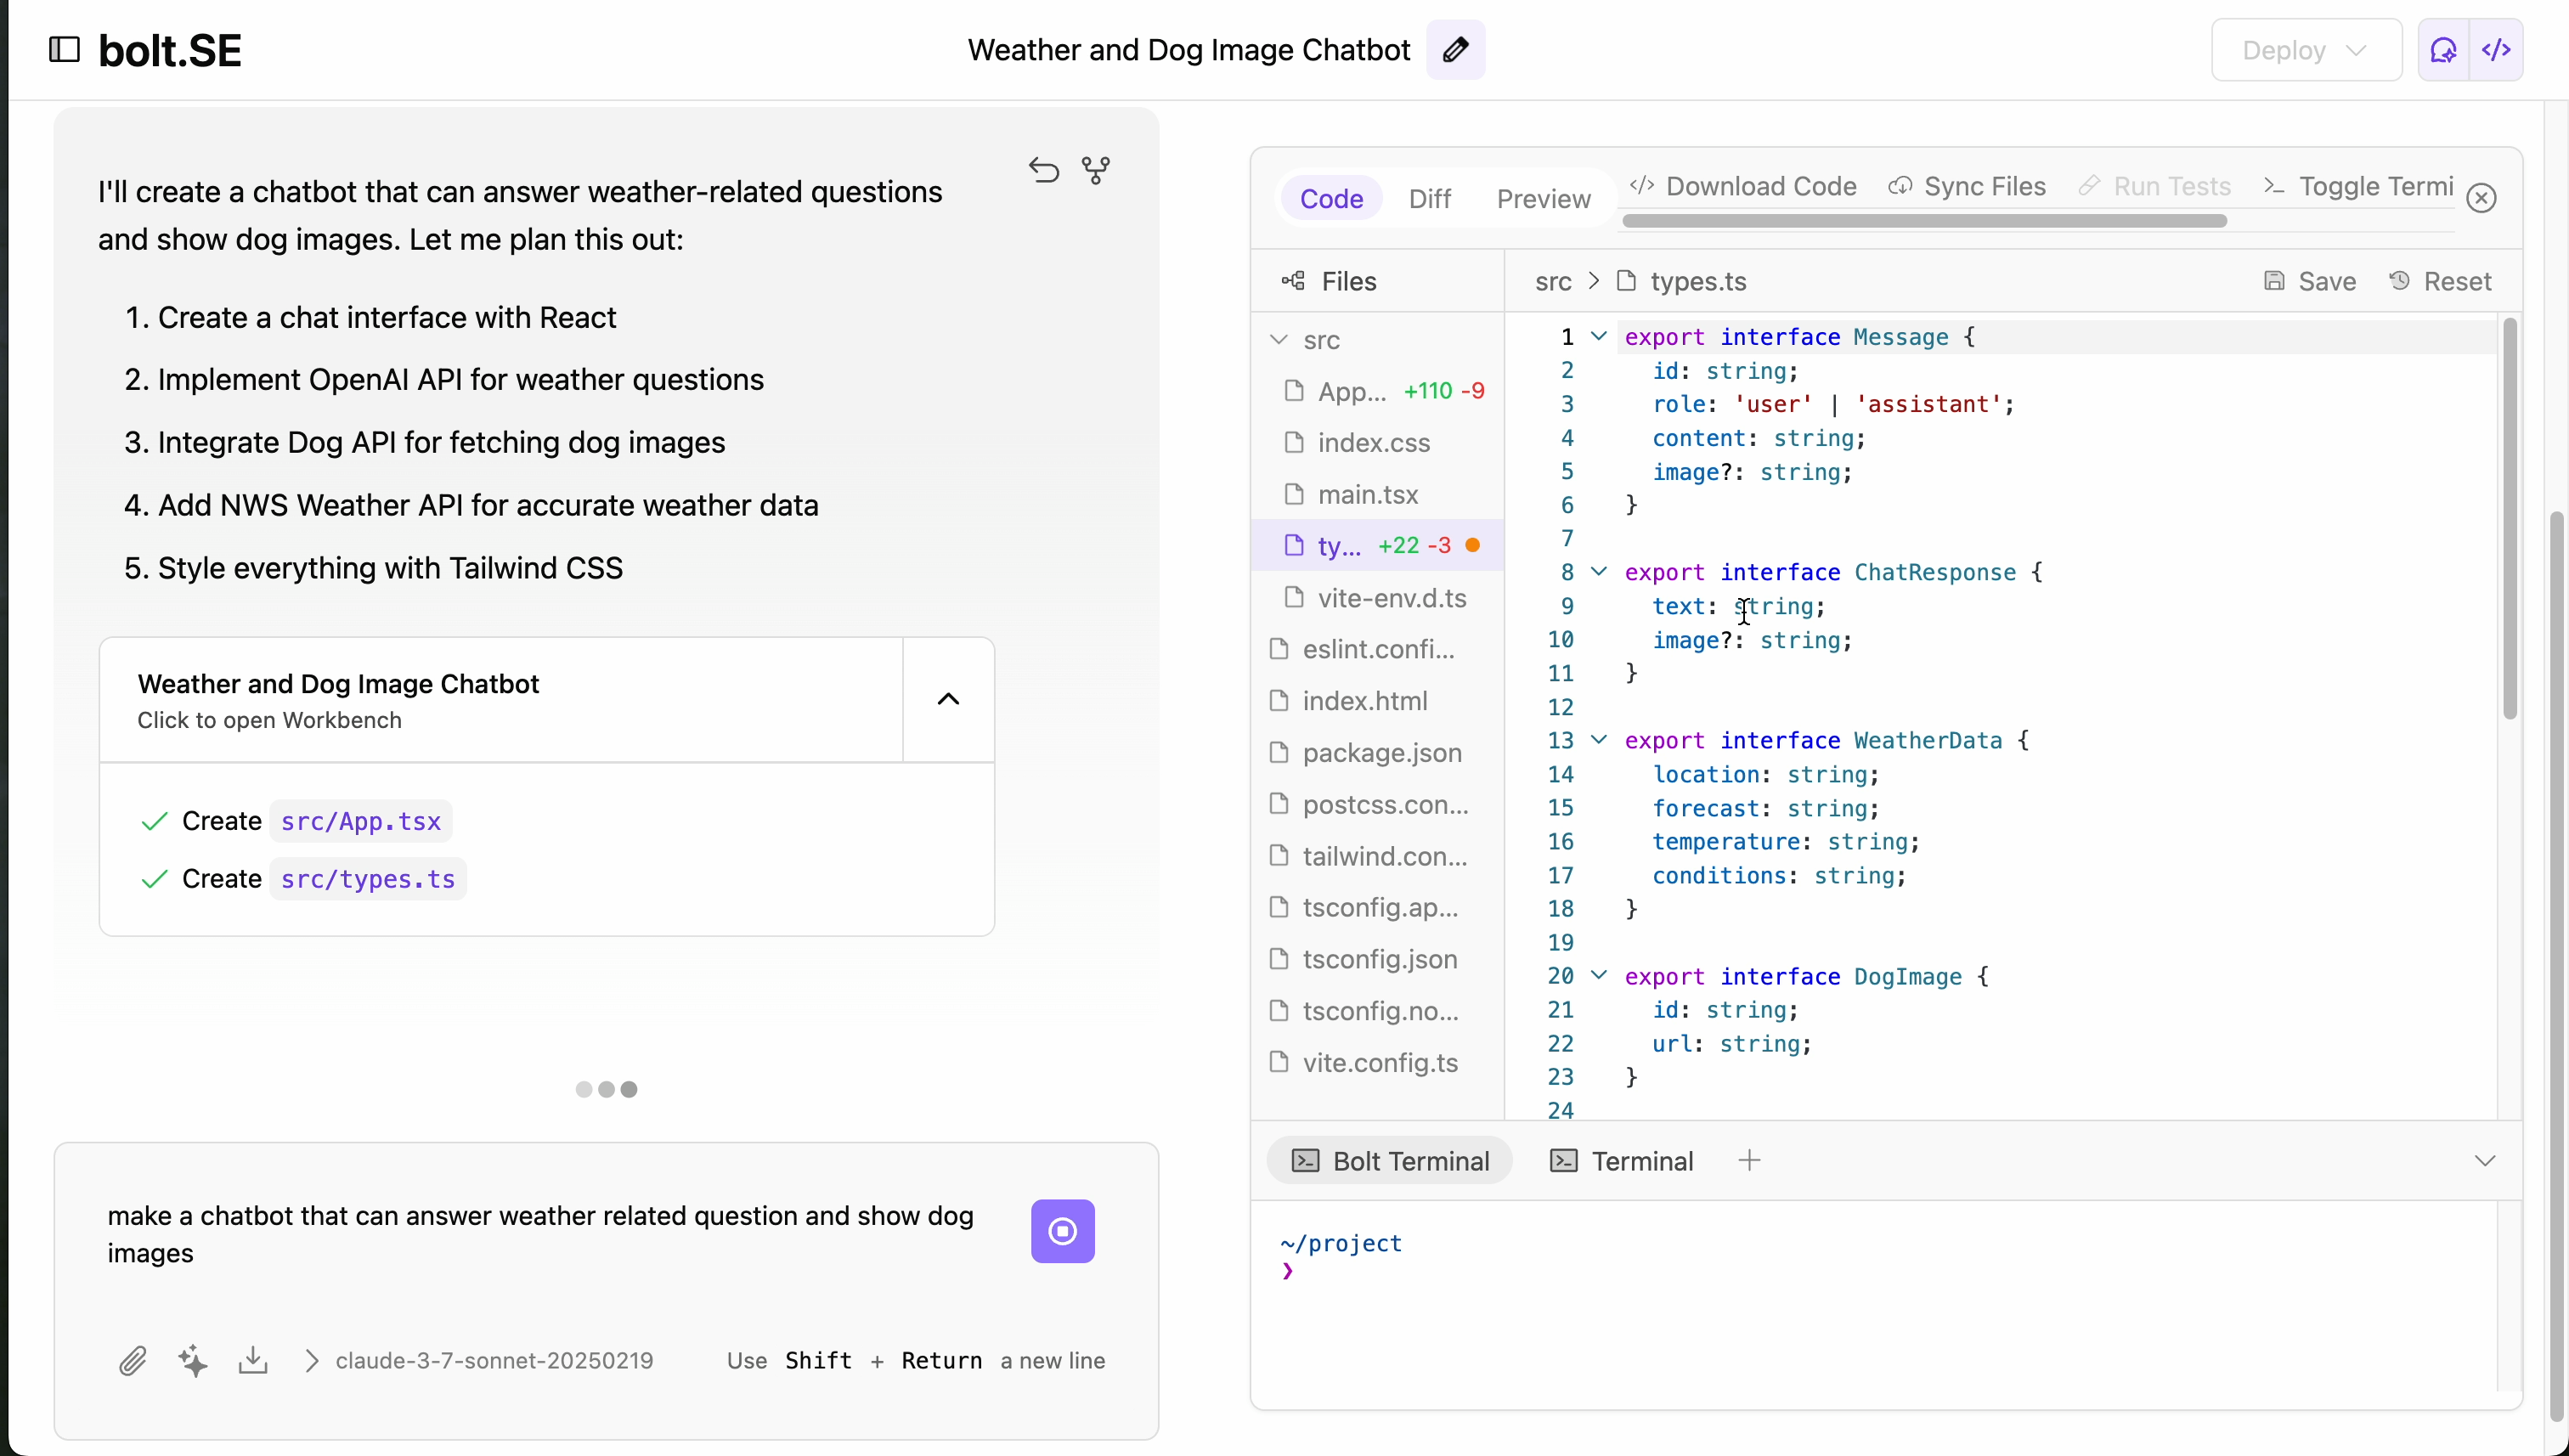
\includegraphics[width=\textwidth]{figures/screenshots/api-actions/demo_plan_files.png}
  \caption{系统生成项目结构与依赖安装命令,覆盖前端组件与服务调用逻辑。}
  \label{fig:demo_plan}
\end{figure}

\subsection{交互效果与 API 调用验证}

在预览界面中,用户可以实时测试机器人功能:

\begin{figure}[htbp]
  \centering
  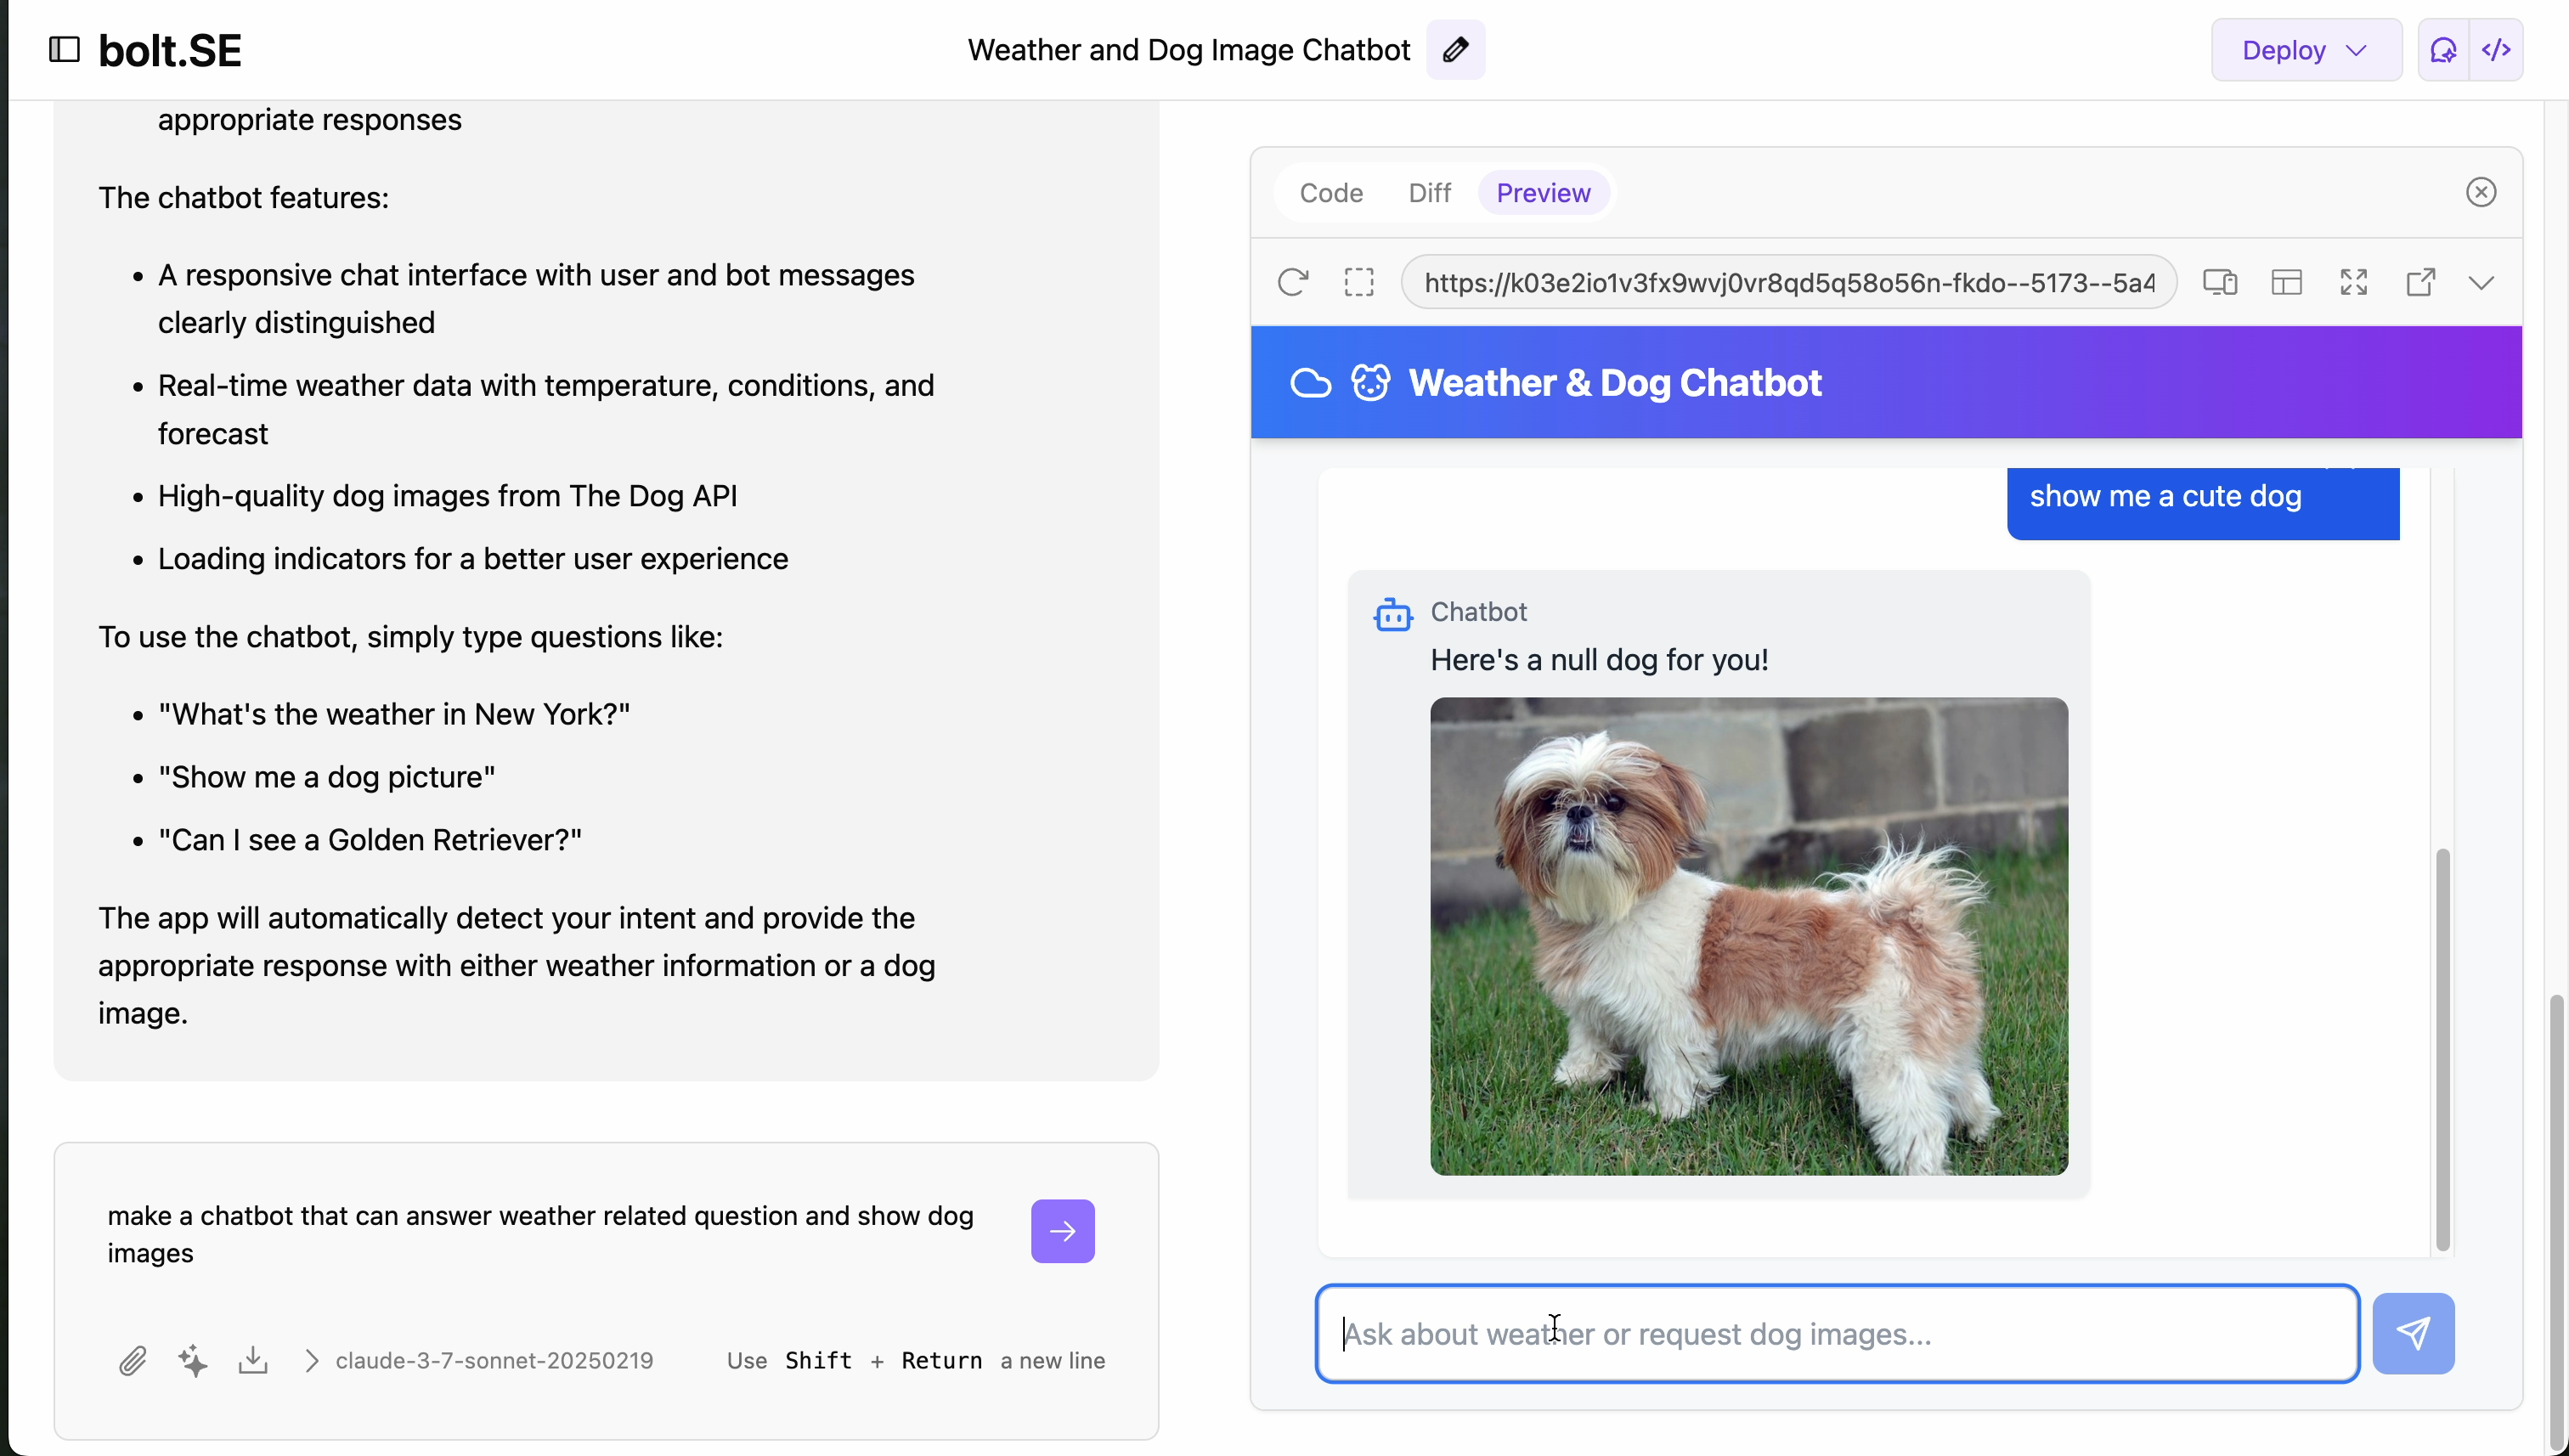
\includegraphics[width=\textwidth]{figures/screenshots/api-actions/demo_dog_preview.png}
  \caption{用户请求"show me a cute dog",系统调用 The Dog API 返回图片。}
  \label{fig:demo_dog}
\end{figure}

\begin{figure}[htbp]
  \centering
  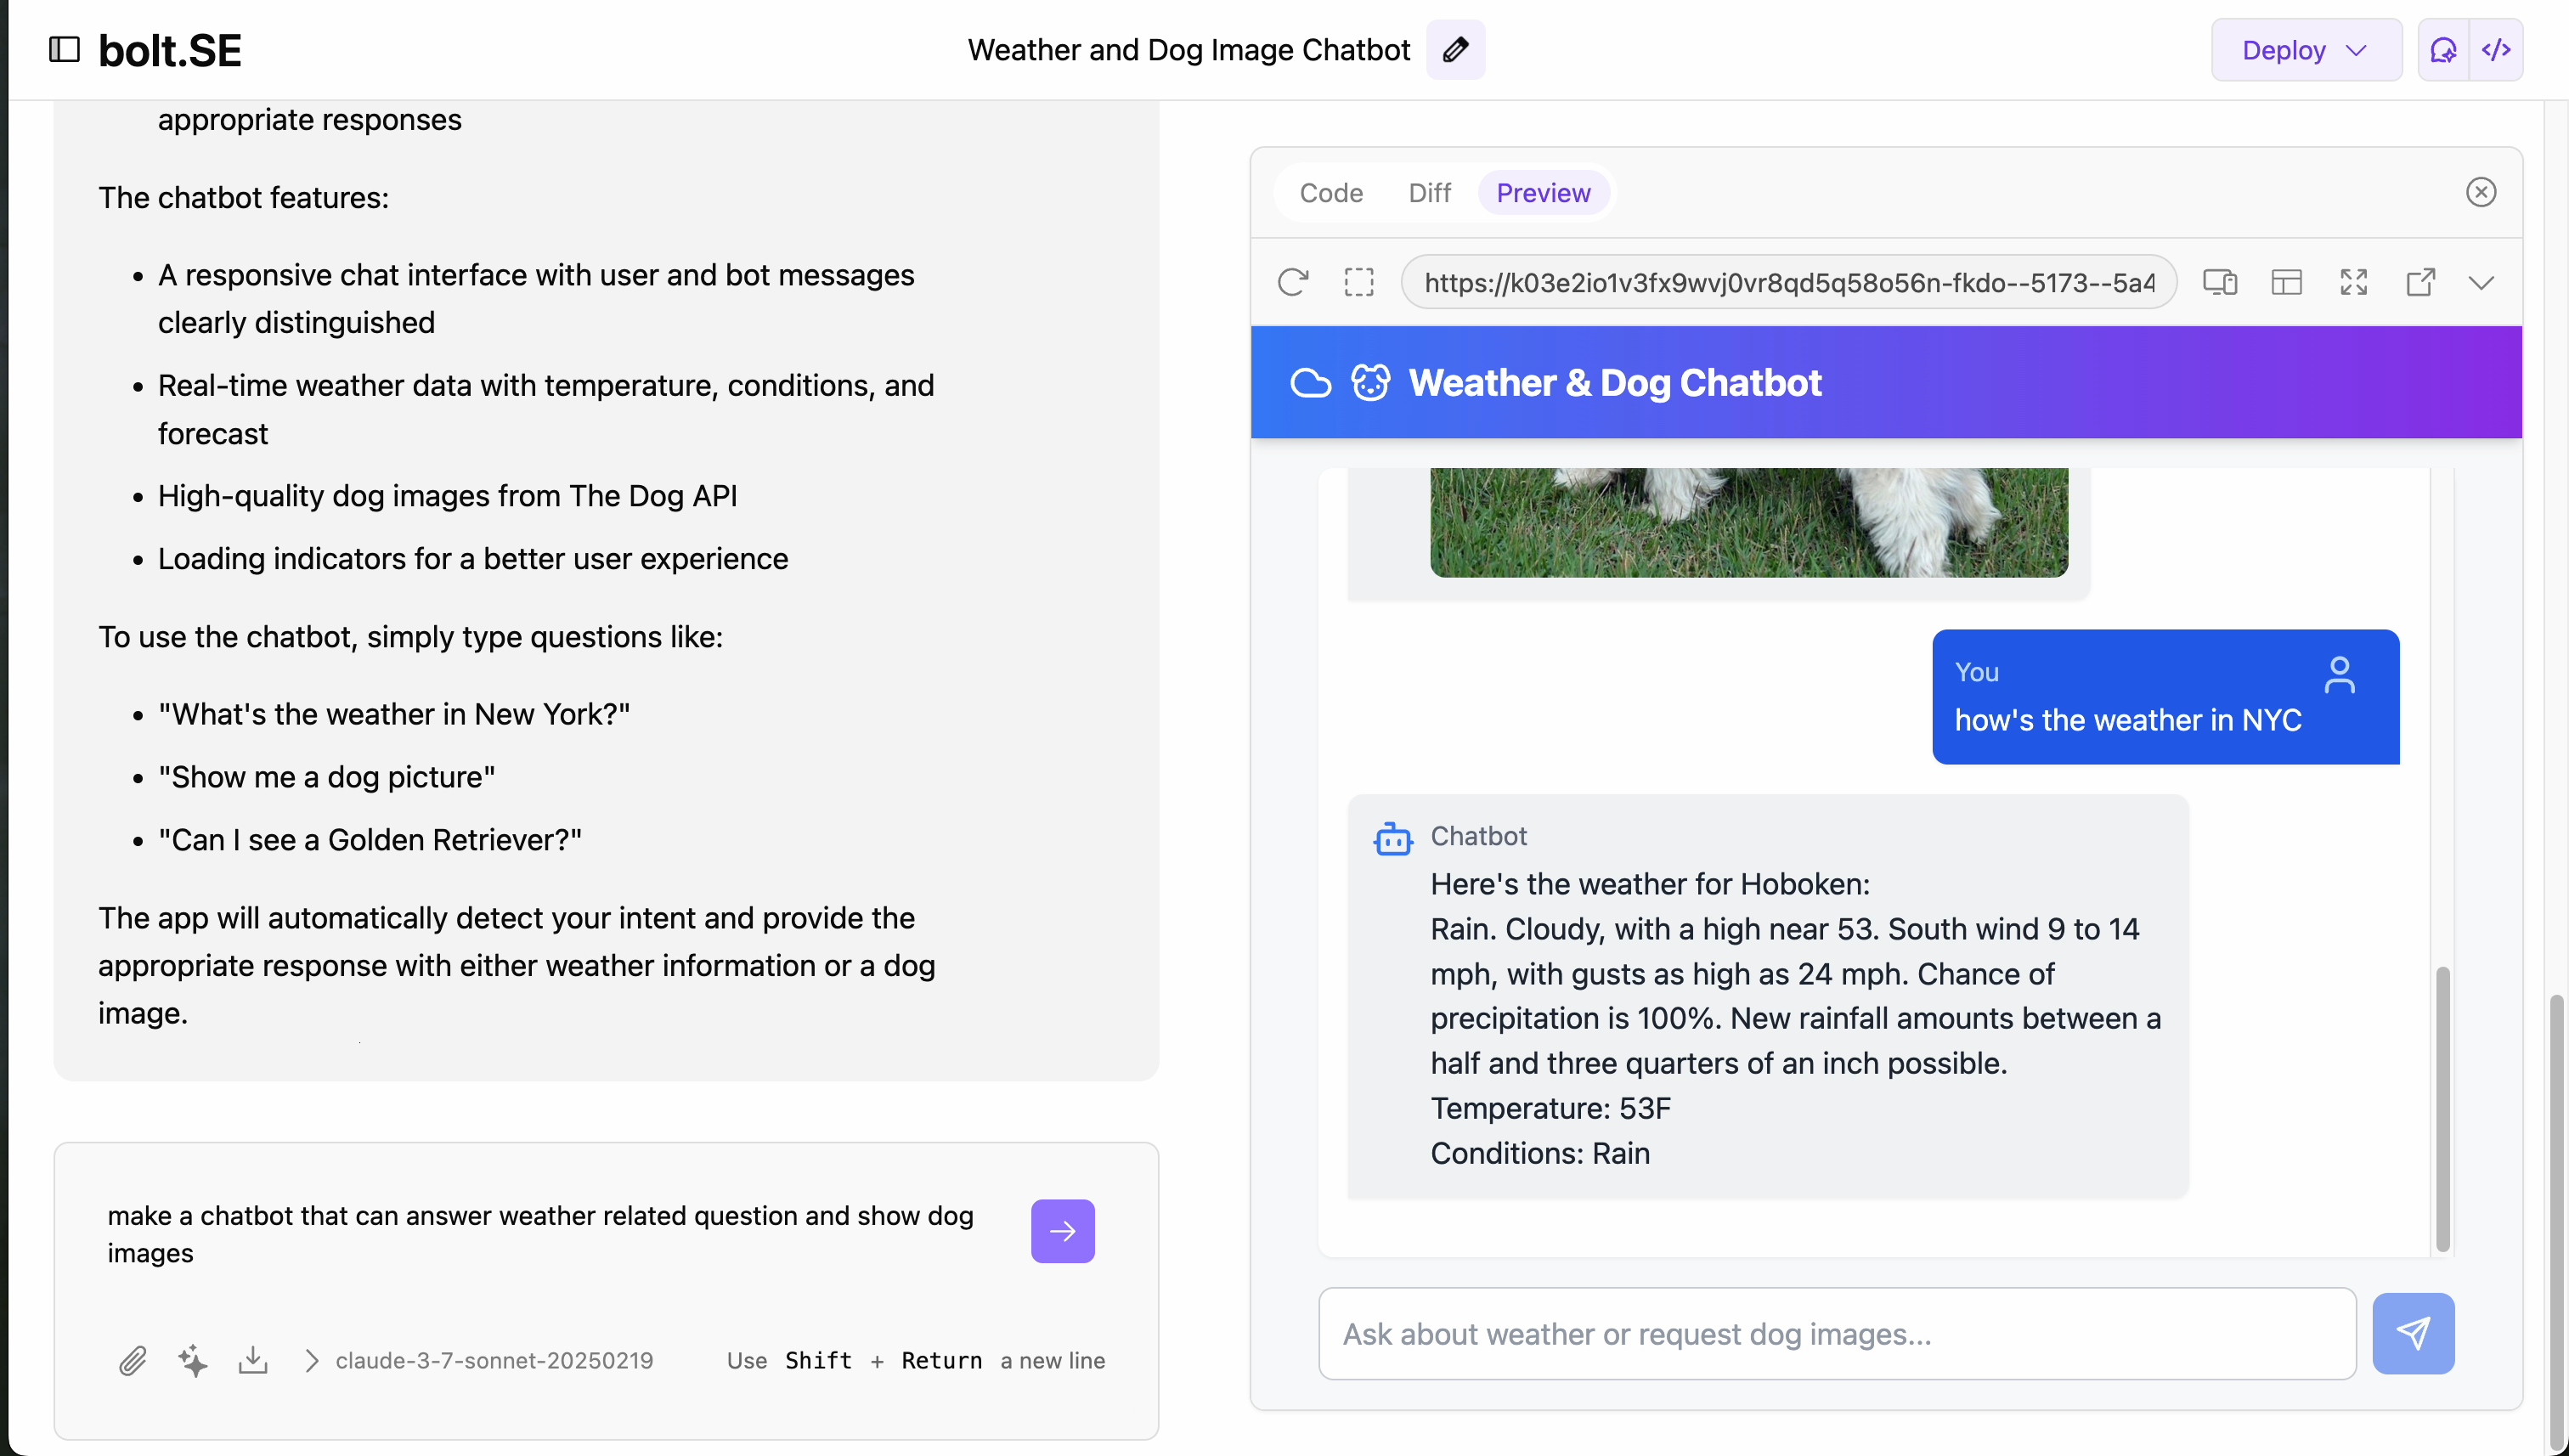
\includegraphics[width=\textwidth]{figures/screenshots/api-actions/demo_weather_preview.png}
  \caption{询问天气时,系统识别意图并调用 NWS Weather API 提供实时天气信息。}
  \label{fig:demo_weather}
\end{figure}

从图中可以看出,聊天机器人能够准确地识别用户意图,
并将意图转化为对外部 API 的调用,展示了 APIActions 与 LLM 的协同优势。

\subsection{与传统开发方式对比}

API优先开发方式与传统开发方式相比具有显著优势:

\begin{itemize}
  \item \textbf{集成效率}:传统开发需要手动编写API调用代码与参数处理逻辑,而APIActions仅需粘贴OpenAPI文档即可自动生成。
  
  \item \textbf{token节省}:结构化API定义避免了冗长自然语言说明,显著降低上下文长度。OpenAPI规范作为结构化格式,比传统开发中使用自然语言描述API功能可节省高达70\%的token消耗。
  
  \item \textbf{开发误差减少}:系统自动完成接口字段绑定,避免了路径拼写、参数顺序或认证机制的人工错误。
  
  \item \textbf{上下文利用率提升}:传统方法中,大量token用于描述API功能和使用方法,而API优先方法通过结构化定义减少了这部分冗余信息,使有限token能够更多地用于实际问题解决。
  
  \item \textbf{减少交互轮次}:由于API定义明确,LLM能够一次性正确理解和使用API,减少了多轮交互纠错,每减少一轮交互可节省数百至数千token。
\end{itemize}

API优先模式在涉及复杂外部服务集成的场景中,不仅提高了开发效率和应用质量,同时通过结构化API描述和减少交互轮次,显著降低了LLM应用的token消耗和运营成本。
